% PocketQuake tutorial — Beamer presentation
% Compile with: pdflatex (or xelatex / lualatex) pocketquake_tutorial.tex
%
% The tutorial guides a first-time user from a fresh clone to the executed
% results notebook of the bundled chungju example. Concise but self-contained:
% every slide has the exact command or path needed.
\documentclass[10pt,aspectratio=169]{beamer}

\usetheme{metropolis}
\usepackage[T1]{fontenc}
\usepackage{graphicx}
\usepackage{listings}
\usepackage{xcolor}

\definecolor{pqorange}{HTML}{D35400}
\definecolor{pqgray}{HTML}{555555}
\setbeamercolor{frametitle}{bg=pqorange,fg=white}
\setbeamercolor{title}{fg=pqorange}

\lstset{
  basicstyle=\ttfamily\scriptsize,
  breaklines=true,
  frame=single,
  framesep=4pt,
  framerule=0.2pt,
  rulecolor=\color{pqgray},
  backgroundcolor=\color{black!3},
  showstringspaces=false,
  keywordstyle=\color{pqorange}\bfseries,
  commentstyle=\color{pqgray}\itshape,
}

% Keep \pqversion in sync with pocketquake.__version__ (single source of truth).
\newcommand{\pqversion}{1.10.0}
\title{PocketQuake}
\subtitle{From a catalog CSV to a relocation notebook in one command}
\author{Min-Seong Seo / SGTL, SNU}
\date{Version \pqversion\ \textbar\ Updated \today}

\begin{document}

\maketitle

% ----------------------------------------------------------------- intro
\begin{frame}[fragile]{What is PocketQuake?}
A thin orchestrator that takes a list of earthquakes and produces a
relocation + focal-mechanism notebook. It glues two specialised submodules:
\begin{itemize}
  \item \textbf{seismoseo/necis-downloader} --- KMA NECIS waveform fetcher
        (Playwright + the FTP staging server).
  \item \textbf{seismoseo/korea-cluster-relocation} --- the picking +
        HypoInverse + HypoDD + SKHASH pipeline.
\end{itemize}

\bigskip
\textbf{One command, end to end:}
\begin{lstlisting}
./pocketquake.sh ./examples/chungju/chungju_catalog.csv chungju
\end{lstlisting}
\bigskip
Output: an executed Jupyter notebook with maps, depth sections, and beachball
diagrams for every event you fed in.
\end{frame}

% ----------------------------------------------------------------- workflow
\begin{frame}{Workflow at a glance}
\begin{center}
\small
\textbf{catalog.csv} \\[2pt]
$\Big\downarrow$ \emph{scaffold cluster dir under the eq-cycle submodule} \\[4pt]
\textbf{kma\_waveforms/}\hspace{2em}(NECIS download via Playwright) \\[2pt]
$\Big\downarrow$ \emph{eq-cycle pipeline} \\[4pt]
PhaseNet+ picking $\to$ HypoInverse $\to$ ph2dt $\to$ dt.ct $\to$ xcorr $\to$ dt.cc $\to$ SKHASH \\[4pt]
$\Big\downarrow$ \\
\textbf{03\_results\_<slug>.ipynb} ~--~ map, depth sections, beachballs
\end{center}

\vspace{1em}
You write the catalog and run one command. PocketQuake takes care of dispatching
to the right waveform source, registering the cluster, and executing the
notebook.
\end{frame}

% ----------------------------------------------------------------- prereqs
\begin{frame}[fragile]{Prerequisites}
\begin{description}
  \item[OS] Linux or macOS (bash wrapper; Windows uses WSL)
  \item[glibc] $\geq$ 2.28 \;---\; Ubuntu 20.04+, RHEL/Rocky 8+, Debian 10+.
        CentOS 7 / RHEL 7 are below the line (Playwright fails).
  \item[Python] 3.10+ (pinned by \texttt{environment.yml})
  \item[conda] Miniforge / Miniconda / Mambaforge
  \item[gcc/gfortran] $\geq$ 9.3 (for the compiled externals)
  \item[Disk] $\sim$10 GB (conda env + Chromium + waveforms)
  \item[Network] HTTPS to \texttt{github.com}, \texttt{code.usgs.gov},
        \texttt{conda-forge}, \texttt{necis.kma.go.kr}
\end{description}
\vspace{0.5em}
\textbf{NECIS account} (apply at \url{https://necis.kma.go.kr}, research /
institutional accounts only; approval 1--5 days). \\
\textbf{STP account} is optional --- only for pre-2020 waveforms.
\end{frame}

% ----------------------------------------------------------------- install
\begin{frame}[fragile]{Install \texttt{[1/2]} --- Python environment}
\begin{lstlisting}[language=bash]
# 1. Clone with submodules
git clone --recurse-submodules https://github.com/seismoseo/PocketQuake.git
cd PocketQuake

# 2. Create the conda env (one command does everything Python-side)
conda env create -f environment.yml
conda activate pocketquake

# 3. Editable installs for PocketQuake itself + the NECIS submodule
pip install -e . -e external/necis-downloader

# 4. Playwright Chromium (one-time, ~200 MB)
playwright install chromium

# 5. Credentials
cp .env.example .env
#  then edit NECIS_USER, NECIS_PASS
\end{lstlisting}
\end{frame}

% ----------------------------------------------------------------- externals
\begin{frame}[fragile]{Install \texttt{[2/2]} --- External programs}
PocketQuake's default chain calls these from the shell. None are
pip-installable. Put each binary on \texttt{\$PATH}:

\begin{itemize}
  \item \texttt{hyp1.40} --- HypoInverse (USGS Fortran)
  \item \texttt{ph2dt} + \texttt{hypoDD} --- Waldhauser's HypoDD (Fortran)
  \item \texttt{mseed2sac} --- IRIS converter (C)
  \item \texttt{libarchive} / \texttt{bsdtar} --- already in \texttt{environment.yml}
\end{itemize}
\smallskip
Two research clones reachable by env var:
\begin{lstlisting}[language=bash]
git clone https://github.com/AI4EPS/EQNet.git
echo "EQNET_DIR=$PWD/EQNet" >> ~/PocketQuake/.env

git clone https://code.usgs.gov/esc/SKHASH.git
echo "SKHASH_DIR=$PWD/SKHASH/SKHASH" >> ~/PocketQuake/.env
\end{lstlisting}
\smallskip
Full per-tool source + build instructions:
\textbf{docs/EXTERNAL\_TOOLS.md}.
\smallskip
\footnotesize
\textbf{Pure-Python option (\texttt{--python}):} replaces the Fortran
\texttt{hyp1.40} + \texttt{ph2dt}/\texttt{hypoDD} with HypoSVI\,+\,EikoNet
and \texttt{relocDD-py} --- no Fortran build needed. See the next-but-one slide.
\end{frame}

% ----------------------------------------------------------------- catalog format
\begin{frame}[fragile]{Catalog format}
A plain CSV with 10 columns, KST origin times:
\begin{lstlisting}
Year,Month,Day,Hour,Minute,Second,Latitude,Longitude,Magnitude,Depth
2025,2,7,2,35,34,37.14,127.76,3.1,9
2025,2,7,2,54,38,37.14,127.76,1.4,6
2025,2,7,3,49,4,37.14,127.76,1.5,7
2025,2,8,10,13,23,37.14,127.76,1.6,7
\end{lstlisting}
\smallskip
\begin{itemize}
  \item Origin time interpreted as KST (UTC + 9 h)
  \item PocketQuake auto-derives the cluster epicenter (catalog centroid)
        and the spatial bounds (bbox + 0.2$^\circ$); override with
        \texttt{--epi}, \texttt{--bounds}
  \item Magnitude is informational --- relocation does not use it
  \item Depth $\geq 0$, measured in km
\end{itemize}
\end{frame}

% ----------------------------------------------------------------- run
\begin{frame}[fragile]{Run the chungju example}
\begin{lstlisting}[language=bash]
./pocketquake.sh ./examples/chungju/chungju_catalog.csv chungju
\end{lstlisting}
\smallskip
The wrapper:
\begin{enumerate}
  \item scaffolds a cluster dir under
        \texttt{external/korea-cluster-relocation/chungju\_cluster/}
  \item downloads NECIS waveforms (Playwright drives the JS portal,
        polls the staging queue, streams the FTP files)
  \item runs PhaseNet+ $\to$ HypoInverse $\to$ HypoDD $\to$ SKHASH
  \item builds + executes the results notebook
\end{enumerate}
\smallskip
Useful flags:
\begin{itemize}
  \item \texttt{--python} --- pure-Python relocation backend (no Fortran; next slide)
  \item \texttt{--source mixed} --- per-event STP+NECIS dispatch
  \item \texttt{--picker stead} --- SeisBench PhaseNet (no EQNet needed)
  \item \texttt{--mainshock <UTC>} --- Gwangyang-style mainshock treatment
  \item \texttt{--cores N} --- cap xcorr workers (default 10)
  \item \texttt{--xcorr-backend} --- dt.cc xcorr kernel (default \texttt{cctorch\_gpu\_batched}, a bit-exact GPU FFT backend that auto-falls-back to obspy without a GPU)
\end{itemize}
\end{frame}

% ----------------------------------------------------------------- pure-python backend
\begin{frame}[fragile]{Pure-Python backend (\texttt{--python})}
A Fortran-free relocation chain that drops in for \texttt{hyp1.40} + \texttt{hypoDD}:
\begin{itemize}
  \item \textbf{HypoSVI + EikoNet} --- absolute location by Stein variational
        inference over a neural-network travel-time field (pretrained weights shipped).
  \item \textbf{relocDD-py} --- Katherine Biegel's Python port of \texttt{hypoDD}
        for the double-difference relocation.
\end{itemize}
\smallskip
One-time setup (no compiler) --- clone the three tools, fetch the weights:
\begin{lstlisting}[language=bash]
git clone https://github.com/katie-biegel/relocDD-py.git
git clone https://github.com/Ulvetanna/HypoSVI.git
git clone https://github.com/Ulvetanna/EikoNet.git
cat >> ~/PocketQuake/.env <<ENV
RELOCDD_PY_DIR=$PWD/relocDD-py
HYPOSVI_DIR=$PWD/HypoSVI
EIKONET_DIR=$PWD/EikoNet
ENV
python -m pipeline.core.fetch_eikonet   # pretrained kim1983 + kim2011
\end{lstlisting}
\smallskip
\begin{lstlisting}[language=bash]
./pocketquake.sh ./examples/chungju/chungju_catalog.csv chungju --python
\end{lstlisting}
\smallskip
\footnotesize
Faithful to the Fortran chain: relative locations match \texttt{hypoDD} to
$\sim$1\,m on identical input; same SVD$\to$LSQR auto-fallback with adaptive
condition-number damping, and the same bootstrap 95\% error bars. The absolute
epicentre can differ (HypoSVI vs HypoInverse) --- that centroid offset is expected.
\end{frame}

% ----------------------------------------------------------------- progress
\begin{frame}[fragile]{What you see while it runs}
\textbf{Foreground} (\texttt{--fg}): full log to terminal. \\
\textbf{Default} (background): \texttt{nohup.out} in the working directory.
\bigskip
\begin{lstlisting}[language=bash]
[pocketquake] scaffolding chungju_cluster ...
[necis] login OK; submitting request for 4 event(s)
[necis] request id 4f3a... status=P -> C, downloading 4 SAC bundles
[eqcycle] picking with phasenet_plus (~30s/event)
[eqcycle] hypoinverse: 4 events located
[eqcycle] xcorr 6 pairs (10 workers) ...
[eqcycle] dt.cc -> hypoDD reloc OK (4 events)
[eqcycle] focal_mechanism: 4 SKHASH solutions
[pocketquake] executing 03_results_chungju.ipynb
\end{lstlisting}
\smallskip
Wall-clock for chungju: $\sim$15 min on a 16-core box.
\end{frame}

% ----------------------------------------------------------------- output 1
\begin{frame}{Output 1 --- Relocated map + focal mechanisms}
\begin{center}
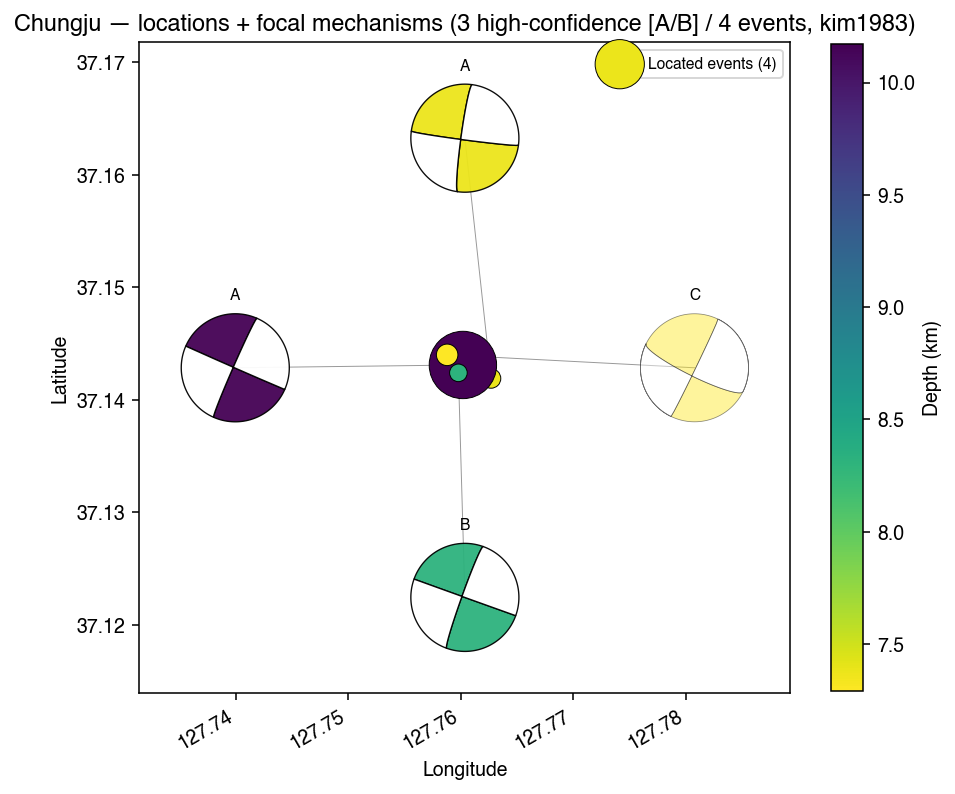
\includegraphics[width=0.85\textwidth,height=0.72\textheight,keepaspectratio]{figures/01_map_mechanisms.png}
\end{center}
\vspace{-0.5em}
\scriptsize
Four located events (depth-coloured dots) at $(37.142^\circ\mathrm{N}, 127.760^\circ\mathrm{E})$
with quality A/B/C SKHASH beachballs drawn on a leader-line ring.
All four solutions converge on a near-vertical N--S right-lateral strike-slip plane.
\end{frame}

% ----------------------------------------------------------------- output 2
\begin{frame}{Output 2 --- Depth sections}
\begin{center}
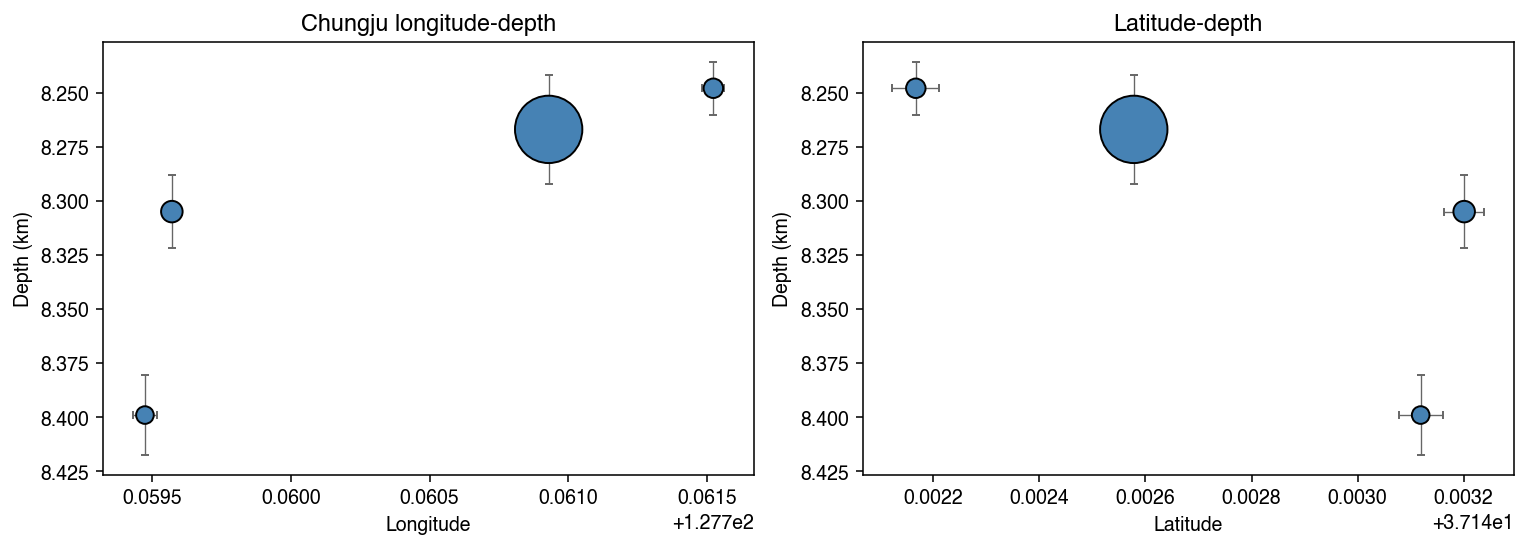
\includegraphics[width=0.8\textwidth]{figures/03_depth_sections.png}
\end{center}
\vspace{-0.5em}
\scriptsize
Three orthogonal cross-sections (E--W, N--S, along-strike) showing the depth
distribution. HypoDD relative-relocation tightens the cluster from
$\sim$1\,km scatter (KMA bulletin) to $\sim$200\,m.
\end{frame}

% ----------------------------------------------------------------- output 3
\begin{frame}{Output 3 --- Beachball gallery + record section}
\begin{columns}[T,onlytextwidth]
\column{0.48\textwidth}
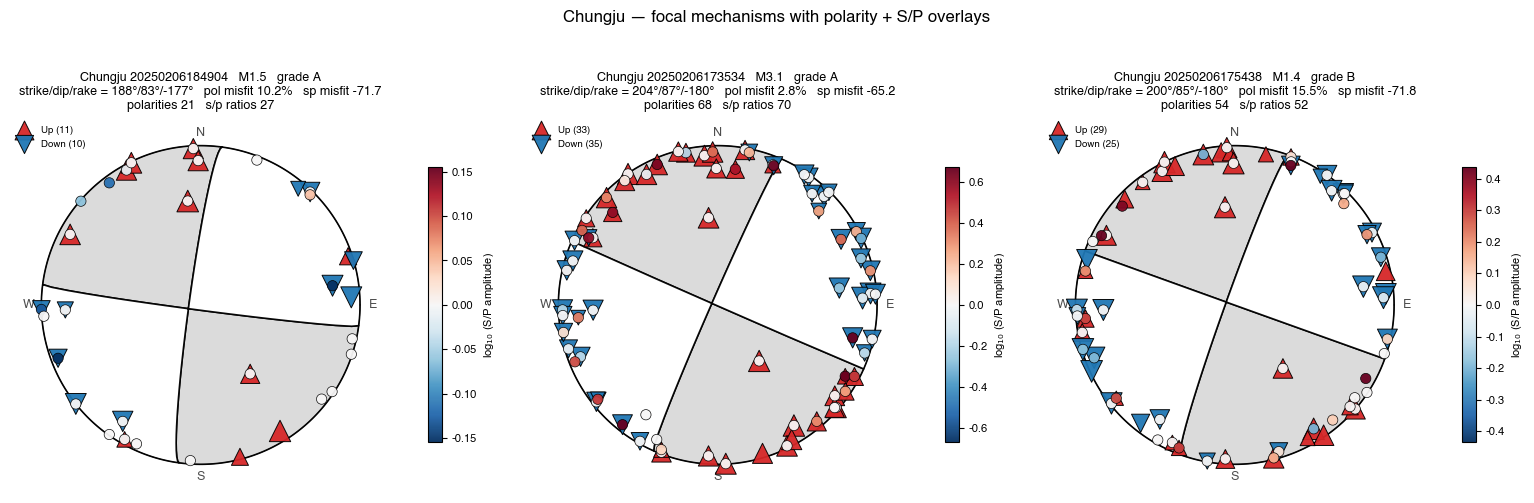
\includegraphics[width=\textwidth]{figures/04_beachball_gallery.png}
\column{0.48\textwidth}
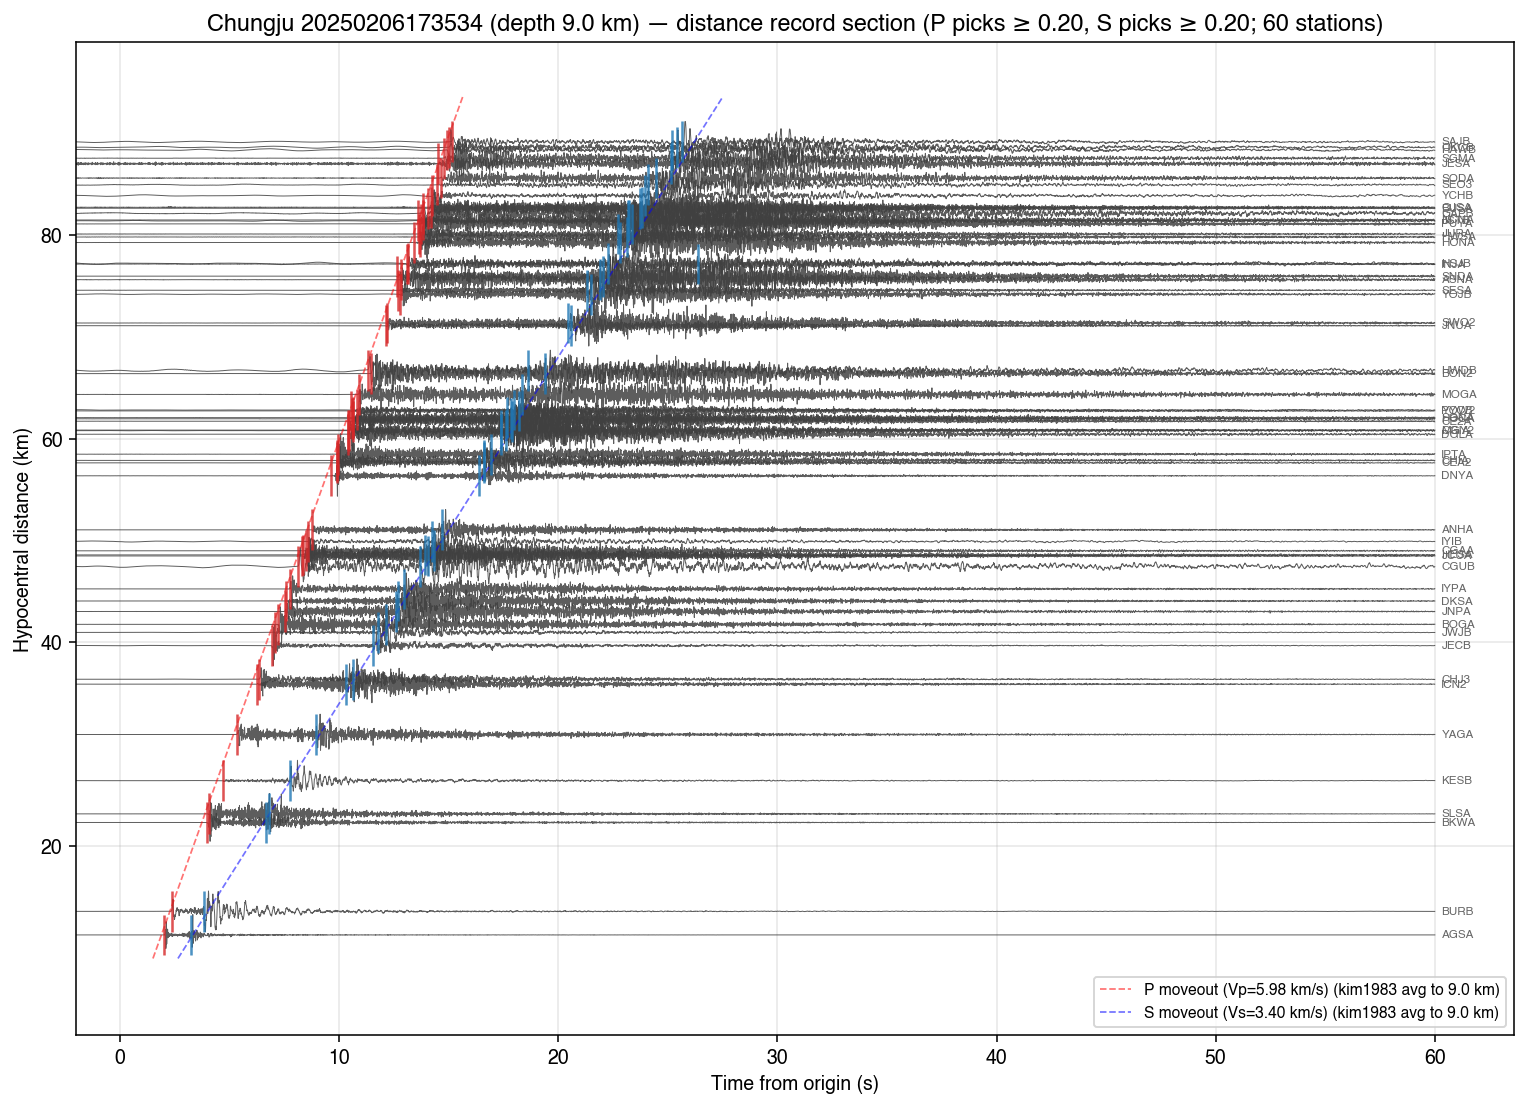
\includegraphics[width=\textwidth]{figures/06_record_section_M31.png}
\end{columns}
\vspace{0.5em}
\scriptsize
The notebook bundles a per-event beachball gallery (left) and a record-section
view of the M3.1 mainshock with PhaseNet+ pick markers, first-motion polarities,
and the SKHASH-inferred S/P amplitude ratios (right).
\end{frame}

% ----------------------------------------------------------------- run own
\begin{frame}[fragile]{Run on your own catalog}
\begin{enumerate}
  \item Save your KMA-style CSV (the format from slide 6).
  \item One command:
\begin{lstlisting}[language=bash]
./pocketquake.sh ~/my_catalog.csv myswarm
\end{lstlisting}
  \item Override the auto-derived epicenter / bounds if your catalog spans
        a wide region:
\begin{lstlisting}[language=bash]
./pocketquake.sh ~/my_catalog.csv myswarm \
    --epi 35.46,128.43 \
    --bounds 35.3,35.65,128.25,128.65
\end{lstlisting}
  \item Mainshock treatment (re-runs xcorr$\to$dt.cc with the mainshock
        excluded, builds a \texttt{\_main} notebook):
\begin{lstlisting}[language=bash]
./pocketquake.sh ~/my_catalog.csv myswarm \
    --mainshock 20240912144719
\end{lstlisting}
\end{enumerate}
\end{frame}

% ----------------------------------------------------------------- options reference
\begin{frame}[fragile]{Command-line options (\texttt{./pocketquake.sh -{}-help})}
\footnotesize
\begin{description}
  \item[\texttt{-{}-python}] pure-Python backend (HypoSVI + relocDD-py; no Fortran)
  \item[\texttt{-{}-compare}] run Fortran \emph{and} Python on the same picks $\to$ side-by-side notebook
  \item[\texttt{-{}-source necis\,|\,stp\,|\,mixed}] waveform source (default \texttt{necis}; use
        \texttt{stp}/\texttt{mixed} for \textbf{pre-2020} events)
  \item[\texttt{-{}-skip-download}] reuse waveforms already on disk (skip the slow download)
  \item[\texttt{-{}-skip-pipeline}] scaffold + download only (no relocation / notebook)
  \item[\texttt{-{}-mainshock <UTC>}] add Gwangyang-style mainshock treatment (\texttt{\_main} notebook)
  \item[\texttt{-{}-picker phasenet\_plus\,|\,stead}] picker model (\texttt{stead} needs no EQNet)
  \item[\texttt{-{}-velmodel kim1983\,|\,kim2011}] velocity model for relocation + focal mech + notebook
  \item[\texttt{-{}-cores N}] cap xcorr workers (default $\sim$10)
  \item[\texttt{-{}-epi},\,\texttt{-{}-bounds}] override the auto-derived epicenter / region
  \item[\texttt{-{}-fg}] foreground (default: background, logs to \texttt{<slug>\_run.log})
\end{description}
\smallskip
\textbf{Velocity model:} location always computes both kim1983 + kim2011; \texttt{-{}-velmodel}
(default kim1983) selects which drives the relocation + focal mechanisms + notebook. Fully for
the Fortran path; with \texttt{-{}-python}, HypoSVI keeps its bundled EikoNet weights.
\end{frame}

% ----------------------------------------------------------------- troubleshooting
\begin{frame}[fragile]{Common pitfalls (\texttt{docs/TROUBLESHOOTING.md})}
\begin{description}
  \item[\texttt{python interpreter not found}] set
        \texttt{POCKETQUAKE\_PYTHON=/path/to/python} in \texttt{.env}
        or put \texttt{python3} on \texttt{\$PATH}.
  \item[\texttt{Permission denied (publickey)}] use the HTTPS clone URL,
        not SSH.
  \item[\texttt{Submodule path '...' not registered}] you forgot
        \texttt{--recurse-submodules}; fix with
        \texttt{git submodule update --init --recursive}.
  \item[\texttt{EQNET\_DIR not set}] PhaseNet+ is the default picker;
        either install EQNet (slide 5) or pass \texttt{--picker stead}.
  \item[\texttt{libstdc++ version not found}] glibc/libstdc++ too old
        (CentOS 7); upgrade OS or run the NECIS download elsewhere.
  \item[\texttt{NECIS\_USER empty}] fill in \texttt{.env}.
\end{description}
\end{frame}

% ----------------------------------------------------------------- end
\begin{frame}{Where to go next}
\begin{itemize}
  \item \textbf{Read the executed result notebook} ---
        \texttt{external/korea-cluster-relocation/pipeline/notebooks/03\_results\_<slug>.ipynb}
  \item \textbf{Inspect the auto-derived configuration} ---
        \texttt{external/korea-cluster-relocation/pipeline/clusters/<slug>.py}
  \item \textbf{Tune the run} --- \texttt{./pocketquake.sh --help}
  \item \textbf{Other examples bundled} --- \texttt{examples/sangju/},
        \texttt{examples/chungju/}, the cluster modules registered in
        \texttt{korea-cluster-relocation/pipeline/clusters/}
  \item \textbf{Docs} --- \texttt{docs/INSTALL.md},
        \texttt{docs/EXTERNAL\_TOOLS.md},
        \texttt{docs/TROUBLESHOOTING.md}
\end{itemize}
\vspace{1em}
\centering
\textbf{\url{https://github.com/seismoseo/PocketQuake}} \\
\smallskip
\textit{Made by Min-Seong Seo / SGTL, SNU.}
\end{frame}

\end{document}
